\chapter{Visualising CloudSat and CALIPSO Data}\label{chap:ccplot}

\section{Introducing \ccplot}
\ccplot is a platform-independent command-line program that can plot several
types of data sets stored in CloudSat, CALIPSO, and Aqua MODIS HDF4 and HDF-EOS2
product files (Tab.\,\ref{tab:plot-types}). It is written in the open-source
scripting language
\program{Python} and uses the
\program{matplotlib} plotting library for its output (see also
Section\,\ref{sec:ccplot-components}\,). Some of the most
important features of \ccplot are:

\begin{itemize}
\setlength{\itemsep}{0pt}
\setlength{\parskip}{0pt}
\setlength{\parsep}{0pt}
\item Support for a number of profile, layer, and swath products.
\item Output in arbitrary quality, fine structure of data can be preserved.
\item Region to be plotted can be selected easily.
\item Suitable for being used by other programs or shell scripts.
\item Colormaps can be customised.
\item Publication-ready output.
\item \ccplot is free software released under the terms of the
open-source-compatible, two-clause BSD license.
\end{itemize}

\begin{table}[h]
\caption[Plot types supported by \ccplot]{\textbf{Plot types supported by \ccplot.}}
\label{tab:plot-types}
\begin{tabular}{p{2.5cm} p{7cm} p{4cm}}
  \sffamily{\textbf{Product}}
& \sffamily{\textbf{Data set}}
& \sffamily{\textbf{\ccplot name}}\\
\tophline

CloudSat 2B-GEOPROF
& Radar Reflectivity Factor
& cloudsat-reflec\\

\middlehline

\multirow{5}{2.5cm}{CALIPSO Lidar L1B Profiles}
& Total Attenuated Backscatter 532nm
& calipso532\\

% empty cell
& Perpendicular Attenuated Backscatter 532nm
& calipso532p\\

% empty cell
& Attenuated Backscatter 1064nm
& calipso1064\\

% empty cell
& Attenuated Color Ratio 1064nm/532nm
& calipso-cratio\\

% empty cell
& Depolarization Ratio
& calipso-dratio\\

\middlehline

\multirow{5}{2.5cm}{CALIPSO Lidar L2 Cloud Layer Products (333m, 1km, 5km)}
& Integrated Attenuated Backscatter 532nm
& calipso532-layer\\

% empty cell
& Integrated Attenuated Backscatter 1064nm
& calipso1064-layer\\

% empty cell
& Integrated Attenuated Total Color Ratio 1064nm/532nm
& calipso-cratio-layer\\

% empty cell
& Integrated Volume Depolarization Ratio
& calipso-dratio-layer\\

% empty cell
& Midlayer Temperature
& calipso-temperature-layer\\

\middlehline

Aqua MODIS L1B, CloudSat, CALIPSO
& MODIS radiance and reflectance;
CloudSat and CALIPSO trajectory
& orbit, orbit-clipped
\end{tabular}
\end{table}


\begin{figure}[t]
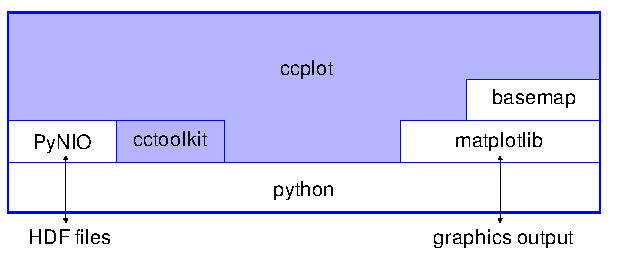
\includegraphics[width=300pt]{images/ccplot-components.pdf}
\caption[Components of \ccplot]{\textbf{Components of \ccplot.} The components that are a
part of the \ccplot code base
are in blue.}
\label{fig:ccplot-components}
\end{figure}

The following sections describe the way \ccplot processes and visualises data.
You may
want to skip right to Chapter\,\ref{chap:ccplot-manual} if you are interested
in how to use \ccplot.


\section{Components of \ccplot}\label{sec:ccplot-components}
As has been mentioned earlier, \ccplot is written in the scripting language
\program{Python}\footnote{\url{http://www.python.org/}}. \program{Python} is a
byte-compiled programming language,
which requires the user to have a copy of the python interpreter installed on
their host system in order to run the program. \program{Python} was chosen for
its suitability for scientific applications thanks to a set of libraries
\program{SciPy}\footnote{\url{http://www.scipy.org/}}, including efficient array
implementation \program{numpy}\footnote{\url{http://numpy.scipy.org/}},
state-of-the-art plotting library
\program{matplotlib}\footnote{\url{http://matplotlib.sourceforge.net/}} and
projection toolkit
\program{basemap}\footnote{\url{
http://matplotlib.sourceforge.net/basemap/doc/html/}}, and a library for reading
HDF files \program{PyNIO}\footnote{\url{http://www.pyngl.ucar.edu/Nio.shtml}}
made by
NCAR (The National Center for Atmospheric Reserch).
To compensate for the
performance-penalty inflicted by the use of a higher-level programming language,
\ccplot uses a set of computationally-intensive functions implemented in C as a
python extension. This extension is called \program{cctk}. The diagram
in Fig.\,\ref{fig:ccplot-components}
shows the relationship between various components of \ccplot.


\begin{figure}[t]
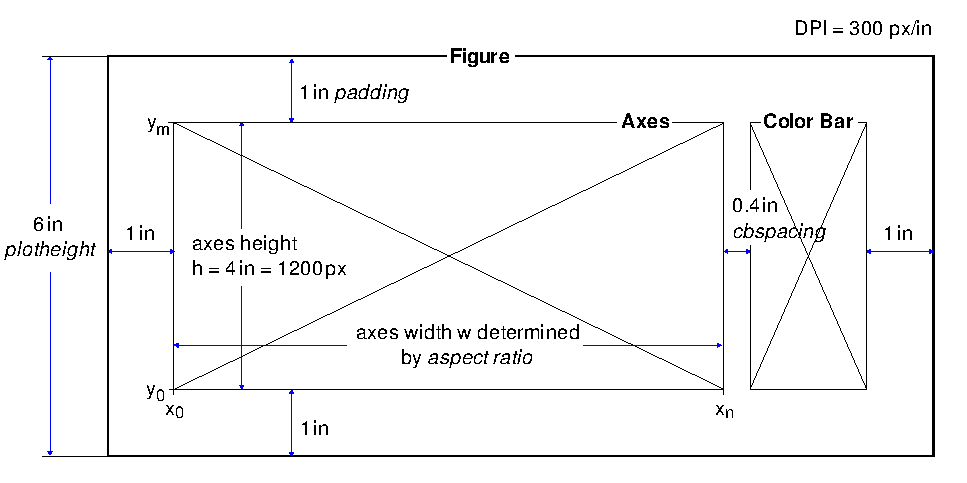
\includegraphics[width=\textwidth]{images/plot-layout2.pdf}
\caption[Plot layout]{\textbf{Plot layout.}
The Figure contains two elements — the Axes and a Color Bar.
The height of the Figure (\textit{plotheight}) is by default \SI{6}{in} regardless of the Axes content.
\SI{1}{in} \textit{padding} on all sides of the Figure results in 4-inch-high Axes,
which translates by DPI\,=\,\SI{300}{px.in^{-1}} to \SI{1200}{px} vertically. $x_0$, $x_n$, $y_0$, $y_m$
are the spatial coordinates of the Axes content. The Axes are by default separated from the Color Bar
by \textit{cbspacing} of \SI{0.4}{in}.
}
\label{fig:plot-layout}
\end{figure}


\section{Data Reading, Processing and Visualisation}

\subsection{Data Reading}
Data are read from data sets in a supplied HDF file. This is done by the
\program{PyNIO} library. After that, dimension mapping is performed, missing
values are masked (so that they are not taken into consideration in later
processing), and data values are converted to scientific values by scaling and
offsetting. Whether and how these operations are performed depends on the type
of the product. For example, dimension mapping is only performed the on MODIS products,
and scaling and offsetting is only performed on the CloudSat products.

The CALIPSO products store height information in a Vdata structure
\textit{metadata}. However, this is not supported by \program{PyNIO} at
the moment, and a temporary solution of storing the height information inside
\ccplot was chosen. This was possible thanks to the fact that the sampling height levels are
constant over all product files.

\subsection{Processing and Visualisation}
\subsubsection{Profile Products}
Profile products are composed of a sequence of rays in the horizontal direction,
and bins in the vertical direction. \ccplot plots profile products on xy-plots,
where the x-axis (horizontal) is linear with rays, and the y-axis (vertical) is
linear with height. Linearity with rays implies linearity with time, because
rays are sampled at a constant frequency of \SI{6.25}{Hz} and
\SI{20.16}{Hz}\footnote{Applies to full resolution products. Others may be
sub-sampled, but rays remain spaced regularly with time.} by CPR and CALIOP
(resp.). Because the A-Train constellation travels at approx. constant velocity
of \SI{7}{km s^{-1}}, the x-axis is also linear with distance travelled.

Because bins are not sampled at regular altitudes, data points have to be
interpolated on a regular grid before being plotted. This is done by the
nearest-neighbour interpolation algorithm described in
Section\,\ref{sec:interpolation-algorithm}\,.
The interpolation only needs to be performed vertically, therefore the
horizontal cut-off radius $r_x = 0$. The vertical cut-off radius $r_y$ is by
default set to an equivalent of \SI{800}{m}, recalculated to pixels according to
the vertical extent, plot height, and DPI\footnote{DPI is the number of pixels
per one inch. Typographical and vector
graphics features of the plot such plot size, font, padding and line widths are
measured in inches, while the profile raster is measured in pixels. DPI is the
size translation factor between these two realms.}:
$$
r_y = \frac{\SI{800}{m}}{y_m - y_0} h \times \mathrm{DPI}
$$

\noindent where $h$ is axes height in inches, and $y_0$ and $y_m$ are the lower and upper boundaries of the
vertical extent (resp.) as introduced in Fig.\,\ref{fig:plot-layout}. Typical bin height is
\SI{30}{m} to \SI{300}{m} for CALIPSO products (Fig.\,\ref{fig:caliop-regions}),
and \SI{240}{m} for CloudSat products (Section\,\ref{sec:atrain-cloudsat}\,). The vertical
cut-off radius of \SI{800}{m} was chosen large in order to err on the safe side.

In the current implementation, the axes height $h$ is by default set to
\SI{4}{in}, and DPI  is by default \SI{300}{px in^{-1}}. This
configuration results in \SI{1200}{px} vertically regardless of the vertical
extent to be plotted. This can be too little to plot all data points if the
vertical extent is large, or unnecessarily much if the vertical extent is small.
One way to mitigate this discrepancy is to increase or decrease (resp.) the plot
height. Another way is to increase or decrease (resp.) DPI, although that may
be restricted by publishing requirements.

\begin{figure}[t]
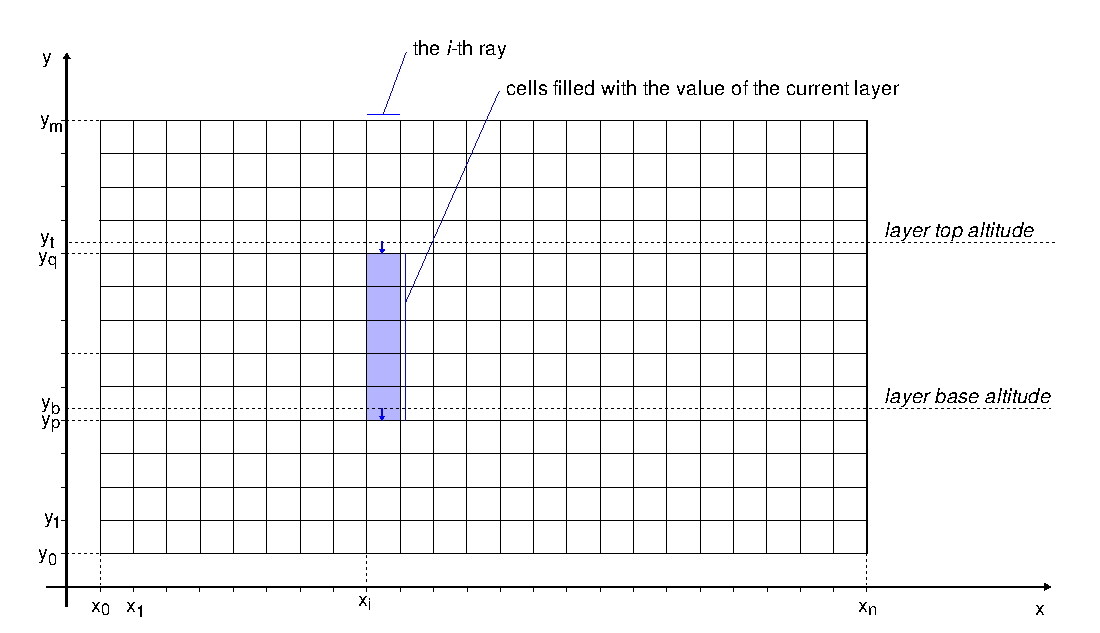
\includegraphics[width=400pt]{images/layermap.pdf}
\caption[The layer mapping algorithm]{\textbf{The layer mapping algorithm.} The algorithm works by iterating
over all layers. Layers are localised by their base and top altitude
$\mathsf{y_b}$ and $\mathsf{y_t}$ (resp.) and
ray number $\mathsf{i}$. The scheme shows a single iteration step. The
coordinates of the low and high cell boundary
$\mathsf{y_p}$, $\mathsf{y_q}$ are calculated by rounding the base and top
altitudes to the nearest horizontal cell boundary.
$\mathsf{(x_0, y_0)}$ and $\mathsf{(x_n, y_m)}$ are the coordinates of the
bottom-left and the upper-right corners of the grid (resp.).}
\label{fig:layermap-algorithm}
\end{figure}


The axes width is determined by the aspect ratio expressed as:
$$
a = \frac{\Delta x_s}{\Delta y_s}
$$
so that an atmospheric feature of a rectangular shape $\Delta x_s \times \Delta
y_s$ is displayed square on the raster. The axes width $w$ in inches is then
calculated as:
$$
w = \frac{h}{a} \frac{x_m - x_0}{y_m - y_0} = \frac{h}{a} \frac{(t_n - t_0)
v_a}{y_m - y_0}
$$
where $x_0$, $x_m$, $y_0$, $y_m$ are as in
Fig.\,\ref{fig:plot-layout}, $t_0$ and $t_n$ are the time of the first ray and the last ray
(resp.), and $v_a$ is the speed of the A-Train constellation, approximated by a
constant of \SI{7}{km s^{-1}}. At $a = 1.0$ atmospheric features may appear
stretched in the horizontal direction, which is caused by the fact that the
horizontal extent of clouds is normally far greater than the vertical extent.
Aspect ratio is by default set to 14.0. If aspect ratio is set equally when
plotting CloudSat and CALIPSO products, the appearance of atmospheric features
is uniform, and therefore easily comparable.

Output fidelity could potentially be increased by taking into consideration that
bins lying higher are shifted backwards horizontally relative to the bins lying
close to the ground, i.e. by calculating the time it takes for a pulse to travel
to a given range and back.


\subsubsection{Layer Products}
Layer products are plotted by filling a regular grid\footnote{Regular with
height in the vertical direction, and with rays in the horizontal direction.}
with data values where there is any atmospheric feature.  Although we could draw
layer features as polygons, we chose not to, because \program{matplotlib} cannot deal with
large amounts of elements effectively. Instead, we use our own simple algorithm
that fills the regular grid, which is then plotted as a raster. The algorithm is
explained graphically in Fig.\,\ref{fig:layermap-algorithm} and in a simplified
pseudo-code in Fig.\,\ref{fig:layermap-algorithm-pseudocode}. The axes size is
determined in the same way as for profile products described in the previous
section.


\subsubsection{Earth View Products and Trajectories}
The Earth View products and trajectories are plotted by translating geographic
coordinates of data and trajectory points into Cartesian coordinates on an
xy-plane by the means of a map projection. This is handled by the
\program{basemap} library. A large set of projections are supported by the
library; however, our experience is that not all projections are properly
implemented, and may fail when asked to translate points that do not lie in the
typical region of the projection.

\begin{table}[t]
\caption[Default values of some parameters in the standard and clipped regimes]{\textbf{Default values of some parameters in the standard and clipped regimes.}}
\label{tab:clipped-parameters}
\begin{tabularx}{\textwidth}{X l l}
			&Clipped		&Not clipped\\
\tophline
Major trajectory ticks	&\SI{1}{min}		&\SI{5}{min}\\
Minor trajectory ticks	&\SI{10}{s}		&\SI{1}{min}\\
Major parallels		&\SI{5}{\degree}	&\SI{30}{\degree}\\
Minor parallels		&\SI{1}{\degree}	&\SI{10}{\degree}\\
Major meridians		&\SI{5}{\degree}	&\SI{30}{\degree}\\
Minor meridians		&\SI{1}{\degree}	&\SI{10}{\degree}
\end{tabularx}
\end{table}

Because Earth View products data points are not positioned regularly with
respect to Cartesian coordinates of any map projection, they have to be
interpolated when they are to be plotted on the xy-plane. To accomplish that,
the nearest-neighbour interpolation algorithm described in
Section\,\ref{sec:interpolation-algorithm}\, is used. Default cut-off radii are
calculated as:
\begin{align}
r_x &= \bigg\lceil \frac{\SI{2000}{m}}{x_n - x_0} w \times \mathrm{DPI}
\bigg\rceil \nonumber\\
r_y &= \bigg\lceil \frac{\SI{2000}{m}}{y_m - y_0} h \times \mathrm{DPI}
\bigg\rceil \nonumber
\end{align}
The value of \SI{2000}{m} was chosen as a large enough value suitable for all three MODIS
resolutions (\SI{250}{m}, \SI{500}{m} and \SI{1}{km}). The cut-off radii can of
course be set manually if any specific value is desired.

The axes height is by default fixed to \SI{4}{in}, and the axes width is
determined according to the aspect ratio reported by \program{basemap}.
Earth View products plotting can operate in two regimes. The standard regime is
not clipped, which causes the entire globe to be plotted. The other regime is
clipped, which sets the projection parameters so that view is clipped
optimally to MODIS swath.  Default values of some other parameters are summarised
in Tab.\,\ref{tab:clipped-parameters}.

Setting central latitude and central meridian, latitude of true scale,
projection centreline, bounding latitude for polar projections, and clipping
region is not supported by the current implementation of \ccplot, but are planned
to be supported by future releases.


%\subsubsection{CloudSat}
%Although the CloudSat mission uses the `self-describing' data format HDF-EOS2
%as
%its base format, the interpretation is not unequivocal, and requires the
%knowledge of additional meta-data. CloudSat deploys the swath
%datatype (Section\,\ref{sec:hdf-eos2}) to store its core data sets. \ccplot
%only supports the
%2B-GEOPROF product in its current implementation, and only the Reflectivity
%Factor data set.
%Apart from the data set to be visualised, \ccplot needs to load the
%global attribute \textbf{\textit{start\_time}} and the following geolocation
%fields:
%\textbf{\textit{Latitude}}, \textbf{\textit{Longitude}},
%\textbf{\textit{Profile\_time}} and \textbf{\textit{Height}}.
%Data from \textbf{\textit{Radar\_Reflectivity}} go through the process of
%masking
%missing values, so that they are not taken into consideration by the
%interpolation algorithm, and through scaling by a defined factor.
%The interpolation algorithm described in
%Section\,\ref{sec:interpolation-algorithm} 
%is used to convert the irregularly distributed data onto a regular grid.
%Time corresponding to a particular ray is calculated by adding
%\textbf{\textit{Profile\_time}} to \textbf{\textit{start\_time}} (in UTC). The
%result is time in UTC, although it may differ from the proper UTC time in the
%rare event when a leap second is introduced in the time period covered by the
%granule.

%\subsubsection{CALIPSO}
%CALIPSO mission files differ from CloudSat and MODIS in a way that they are
%stored in plain HDF4 files (as opposed to HDF-EOS2). The meta-data is more
%scarce, and even some meta-data information of HDF4 such as dimension names is
%not used.
%When \ccplot is instructed to plot a profile data set such as the Total
%Attenuated
%Backscatter 532nm, the fields read are
%\textbf{\textit{Total\_Attenuated\_Backscatter\_532}},
%\textbf{\textit{Latitude}}, \textbf{\textit{Longitude}} and
%\textbf{\textit{Profile\_UTC\_Time}}. The height information is expected to be
%read from the Vdata structure \textbf{\textit{metadata}}. However, this is not
%supported by \program{PyNIO} at the moment, and a temporary solution of storing
%the height information inside \ccplot was chosen. This was possible, because
%the
%height is constant over all product files, although this is not guaranteed by
%the technical documentation, and the issue will need to be addressed soon.
%The only difference in
%processing CALIPSO profiles from CloudSat is that the height field is constant
%in the along-track direction, and is therefore only one-dimensional.

%Plotting layer data types is more involved. The L2 layer products contain
%\textbf{\textit{Longitude}}, \textbf{\textit{Latitude}} and
%\textbf{\textit{Profile\_UTC\_Time}}
%fields similar to profile products, but
%the structure of the other locational fields differs substantially
%(Section\,\ref{sec:hdf-calipso-products}).
%Although we could draw the layers as polygons, we chose not to, because
%\program{matplotlib} cannot deal with large amounts of elements effectively.
%Instead, we
%use our own simple algorithm that fills a regular grid by the layers, and then
%draws the grid as an image. The algorithm is explained graphically in
%Fig.\,\ref{fig:layermap-algorithm}
%and in a simplified pseudo-code in
%Fig.\,\ref{fig:layermap-algorithm-pseudocode}.

\begin{figure}[h]
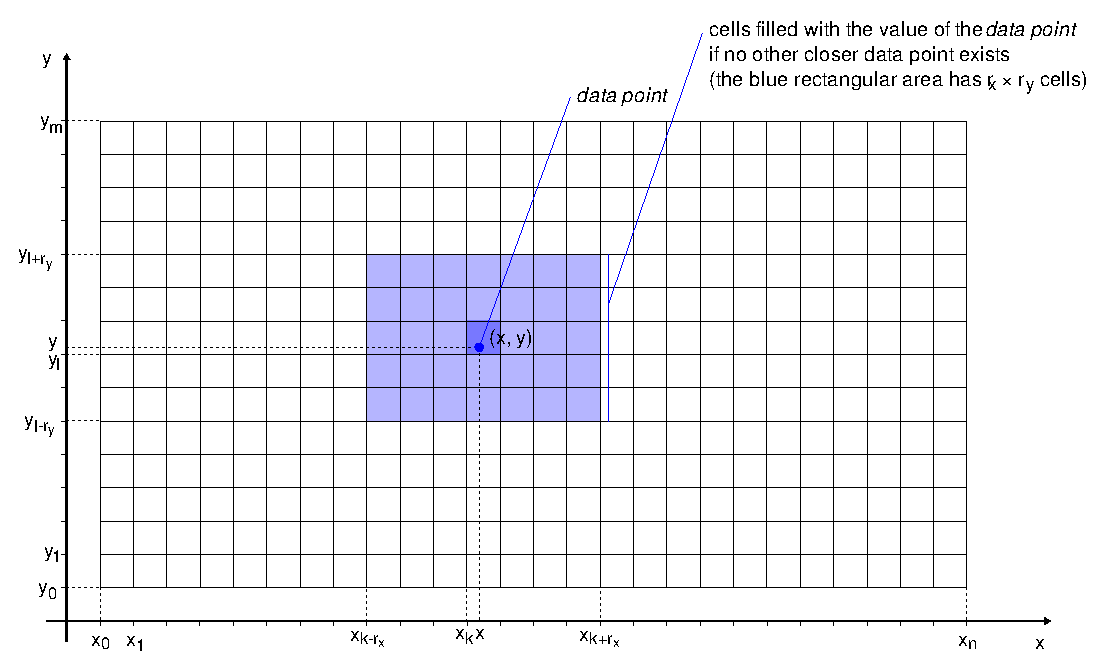
\includegraphics[width=350pt]{images/interpolation.pdf}
\caption[The interpolation algorithm]{\textbf{The interpolation algorithm.} The algorithm works by iterating
over all source data points,
and filling those cells of the regular grid which are within a rectangular area
of $\mathsf{r_x \times r_y}$ cells,
and for which there have been no previous data points lying closer. The distance
is calculated in screen coordinates.
The scheme shows a single iteration step with a \textit{data point} at
$\mathsf{(x, y)}$.
$\mathsf{(r_x, r_y)}$ are the cut-off radii, $\mathsf{(x_k, y_l)}$ are the
coordinates of the cell lying closest to the data point, and
$\mathsf{(x_0, y_0)}$ and $\mathsf{(x_n, y_m)}$ are the coordinates of the
bottom-left and the upper-right corners of the grid (resp.).}
\label{fig:interpolation-algorithm}
\end{figure}

\subsection{The Interpolation Algorithm}\label{sec:interpolation-algorithm}
Data from profile and MODIS swath products are not suitable for direct
visualisation,
because
they are not distributed regularly with respect to desirable coordinates
such as altitude in the vertical, or meters in the horizontal. 
In order to achieve that, we
use a \textit{nearest-neighbour interpolation algorithm} with an amendable
\textit{cut-off radius}
in both directions, so that input samples are not taken as a source for
far-enough points. This
algorithm was used in an effort to present data with minimum distortion.
Fig.\,\ref{fig:interpolation-algorithm} explains the interpolation algorithm by
graphical means, and Fig.\,\ref{fig:interpolation-algorithm-pseudocode}
contains a listing of the interpolation algorithm in a simplified pseudo-code.
The actual implementation has been programmed in C, and as such scales well to
large data sets.


\begin{figure}[h]
\lstset{
	basicstyle=\footnotesize\ttfamily,
	keywordstyle=\bfseries,
	commentstyle=\color{grey},
	frame=single,
	rulecolor=\color{blue},
	framexleftmargin=2pt,
	xleftmargin=6.5pt,
	xrightmargin=4.5pt,
	morecomment=[l]\#,
	morekeywords={for,if,from,to,array,of,return,continue,not}
}

\begin{lstlisting}
# Performs mapping of CALIPSO layer data onto a regular grid.
#
# Arguments:
#
# data[n][U]    - array of data values, where n is the number of rays
#                 and U is the maximum number of layers per ray
# nlayer[n]     - array of number of layers in a ray
# basealt[n][U] - array of layer base altitudes
# topalt[n][U]  - array of layer top altitudes
# y0            - the y-coordinate of the bottom boundary of the grid
# ym            - the y-coordinate of the top boundary of the grid
# m             - number of grid cells in the y- direction
#
layermap(data[n][U], nlayer[n], basealt[n][U], topalt[n][U], y0, ym, m)
    grid[n,m] = array of NaN # The output raster.
                             # NaN stands for Not a Number,
                             # a value indicating an empty cell.

    # For each ray.
    for i from 0 to n-1:
        # For each layer in ray i.
        for j from 0 to nlayer[i]-1:
            yb = basealt[i][j]
            yt = topalt[i][j]
            pf = (yb - y0) / (ym - y0) * m
            qf = (yt - y0) / (ym - y0) * m
            p = round(pf)
            q = round(qf)
            
            for k from p to q-1:
                grid[i][k] = data[i][j]

    return grid
\end{lstlisting}
\caption[The layer mapping algorithm in pseudo-code]{\textbf{The layer mapping algorithm in pseudo-code.}
The algorithm is supplied with a n\texttimes{U} array of scientific values
data[n][U].
Only the first nlayer[i] items of data[i] contain meaningful values.
The output is a regular grid of n\texttimes{m} cells.
Also see Fig.\,\ref{fig:layermap-algorithm} for a graphical explanation of the
layer mapping algorithm.}
\label{fig:layermap-algorithm-pseudocode}
\end{figure}

\begin{figure}[p]
\lstset{
	basicstyle=\footnotesize\ttfamily,
	keywordstyle=\bfseries,
	commentstyle=\color{grey},
	frame=single,
	rulecolor=\color{blue},
	framexleftmargin=2pt,
	xleftmargin=6.5pt,
	xrightmargin=4.5pt,
	morecomment=[l]\#,
	morekeywords={for,if,from,to,array,of,return,continue,not}
}
	

\begin{lstlisting}
# Implementation of the nearest-neighbour interpolation algorithm.
#
# Arguments:
#
# data[N]  - array of N data points
# coord[N] - array of N (x, y) pairs denoting the coordinates of
#            corresponding data points
# x0       - the x-coordinate of the left boundary of the grid
# xn       - the x-coordinate of the right boundary of the grid
# n        - number of grid cells in the x-direction
# y0       - the y-coordinate of the bottom boundary of the grid
# ym       - the y-coordinate of the top boundary of the grid
# m        - number of grid cells in the y-direction
# rx       - cut-off radius in the x-direction
# ry       - cut-off radius in the y-direction
#
interpolate(data[N], coord[N], x0, xn, n, y0, ym, m, rx, ry):
    grid[n][m] = array of NaN # The output raster.
                              # NaN stands for Not a Number,
                              # a value indicating an empty cell.
     
    distance[n][m] = array of +infinity # Distance of the nearest
                                        # data point as would appear
                                        # on the screen.
    
    # Interate over all data points.
    for i from 0 to N-1:
        value = data[i]
        (x, y) = coord[i]
        
        # Position of the data point on the grid.
        kf = (x - x0) / (xn - x0) * n
        lf = (y - y0) / (yn - y0) * m
        k = round(kf)
        l = round(lf)
        
        # For each cell within the cut-off distance.
        for p from -rx to rx:
            for q from -ry to ry:
                u = k + p 
                v = l + q

                if not (0 <= u < n and 0 <= v < m):
                    continue
                
                d = (u - kf)^2 + (v - lf)^2
                if d < distance[u][v]:
                    distance[u][v] = d
                    grid[u][v] = value
    return grid
\end{lstlisting}
\caption[The interpolation algorithm in pseudo-code]{\textbf{The interpolation algorithm in pseudo-code.} The algorithm
takes an array of N input data points described by their value and coordinates,
and parameters of a regular grid.
The output of the algorithm is an {n}\texttimes{m} array — the grid. See also
Fig.\,\ref{fig:interpolation-algorithm} for a
graphical explanation.}
\label{fig:interpolation-algorithm-pseudocode}
\end{figure}
